\documentclass{ximera}

\input{../../../preamble.tex}


\definecolor{fvdnavy}{HTML}{071D43}
\definecolor{fvdcyan}{HTML}{20BFC6}
\definecolor{fvdcyanlight}{HTML}{EFFCFB}
\definecolor{fvdmagenta}{HTML}{F10D69}
\definecolor{fvdmagentalight}{HTML}{FFF1F7}
\definecolor{fvdtext}{HTML}{163044}





%=================================================
% Pedagogische omgevingen
% PDF: tcolorbox
% HTML: learning-box
%=================================================

\newenvironment{voorkennis}
{%
    \ifdefined\HCode
        \HCode{%
<section class="learning-box learning-box--prior">
<div class="learning-box__header">
<span class="learning-box__icon" aria-hidden="true"></span>
<span class="learning-box__title">Voorkennis</span>
</div>
<div class="learning-box__content">
        }%
        \begin{itemize}
    \else
       \begin{tcolorbox}[
    enhanced,
    breakable,
    colback=fvdcyanlight,
    colframe=fvdcyan,
    coltext=fvdtext,
    boxrule=0.5pt,
    leftrule=4pt,
    arc=4mm,
    outer arc=4mm,
    left=7mm,
    right=6mm,
    top=5mm,
    bottom=5mm,
    before skip=6mm,
    after skip=6mm,
    title=Voorkennis,
    coltitle=fvdcyan,
    fonttitle=\bfseries\Large,
    attach title to upper={\par\smallskip},
    boxed title style={
        empty,
        left=0mm,
        right=0mm,
        top=0mm,
        bottom=0mm
    },
    overlay={
        \draw[
            fvdcyan,
            line width=0.5pt
        ]
        ([xshift=42mm,yshift=-13mm]frame.north west)
        --
        ([xshift=-7mm,yshift=-13mm]frame.north east);
    }
]
        \begin{itemize}
    \fi
}
{%
    \end{itemize}
    \ifdefined\HCode
        \HCode{%
</div>
</section>
        }%
    \else
        \end{tcolorbox}
    \fi
}


\newenvironment{leerdoelen}
{%
    \ifdefined\HCode
        \HCode{%
<section class="learning-box learning-box--goals">
<div class="learning-box__header">
<span class="learning-box__icon" aria-hidden="true"></span>
<span class="learning-box__title">Leerdoelen</span>
</div>
<div class="learning-box__content">
        }%
        \begin{itemize}
    \else
\begin{tcolorbox}[
    enhanced,
    breakable,
    colback=fvdmagentalight,
    colframe=fvdmagenta,
    coltext=fvdtext,
    boxrule=0.5pt,
    leftrule=4pt,
    arc=4mm,
    outer arc=4mm,
    left=7mm,
    right=6mm,
    top=5mm,
    bottom=5mm,
    before skip=6mm,
    after skip=6mm,
    title=Leerdoelen,
    coltitle=fvdmagenta,
    fonttitle=\bfseries\Large,
    attach title to upper={\par\smallskip},
    boxed title style={
        empty,
        left=0mm,
        right=0mm,
        top=0mm,
        bottom=0mm
    },
    overlay={
        \draw[
            fvdmagenta,
            line width=0.5pt
        ]
        ([xshift=42mm,yshift=-13mm]frame.north west)
        --
        ([xshift=-7mm,yshift=-13mm]frame.north east);
    }
]
        \begin{itemize}
    \fi
}
{%
    \end{itemize}
    \ifdefined\HCode
        \HCode{%
</div>
</section>
        }%
    \else
        \end{tcolorbox}
    \fi
}



\title{Wanneer is een functie omkeerbaar?}
\author{Ingmar Herreman}

\begin{document}

% FVD_CHAPTER_DATA_START
% Automatisch gegenereerd uit index.tex.
% Niet handmatig aanpassen.
\fvdchapterdata{4}{Van relatie naar functie}{3}
% FVD_CHAPTER_DATA_END









\begin{abstract}
Een functie voert een bewerking uit in één richting:
\[
x\longmapsto f(x).
\]
Maar kunnen we vanuit een functiewaarde altijd eenduidig terugvinden welke
invoerwaarde erbij hoorde?

In dit hoofdstuk onderzoeken we wanneer die terugweg mogelijk is. We bouwen
daarvoor precies de begrippen op die we nodig hebben: \textbf{injectief},
\textbf{surjectief} en vooral \textbf{bijectief}. De grafiek staat centraal:
met horizontale lijnen onderzoeken we hoeveel originelen een functiewaarde heeft.

Dit hoofdstuk vormt de rechtstreekse voorbereiding op de inverse functie.
\end{abstract}

\maketitle

\begin{voorkennis}
    \item Je begrijpt domein, codomein en bereik.
    \item Je kan beelden en originelen bepalen.
    \item Je weet dat één functiewaarde meerdere originelen kan hebben.
    \item Je kan een grafiek lezen en GeoGebra gebruiken om snijpunten te onderzoeken.
\end{voorkennis}

\begin{leerdoelen}
    \item Je kan uitleggen wanneer een functie injectief, surjectief en bijectief is.
    \item Je kan deze eigenschappen herkennen in pijldiagrammen en grafieken.
    \item Je kan de horizontale-lijntest gebruiken en verklaren.
    \item Je kan het verband leggen tussen injectiviteit en het aantal originelen.
    \item Je kan het verband leggen tussen surjectiviteit, bereik en codomein.
    \item Je kan uitleggen waarom bijectiviteit precies de voorwaarde is voor een eenduidige terugweg.
    \item Je kan onderzoeken hoe een beperking van domein of codomein een functie bijectief kan maken.
    \item Je kan GeoGebra doelgericht inzetten om omkeerbaarheid grafisch te onderzoeken.
\end{leerdoelen}



% ============================================================
% 1. DE TERUGWEG
% ============================================================

\FVDsection{Kan je vanuit de uitvoer terug?}

Bij een functie is de voorwaartse richting eenduidig:
\[
x\longmapsto f(x).
\]

Voor iedere toegelaten \(x\) bestaat precies één functiewaarde \(f(x)\).

De omgekeerde vraag is subtieler:
\[
y\longmapsto \text{welke }x\text{ had beeld }y?
\]

\begin{voorbeeld}[Waarom de terugweg kan mislukken]

Beschouw
\[
f(x)=x^2.
\]

Dan geldt
\[
f(-2)=4
\qquad\text{en}\qquad
f(2)=4.
\]

Als we alleen weten dat de uitvoer \(4\) is, kunnen we dus niet eenduidig
beslissen of de oorspronkelijke invoer \(-2\) of \(2\) was.

\begin{center}
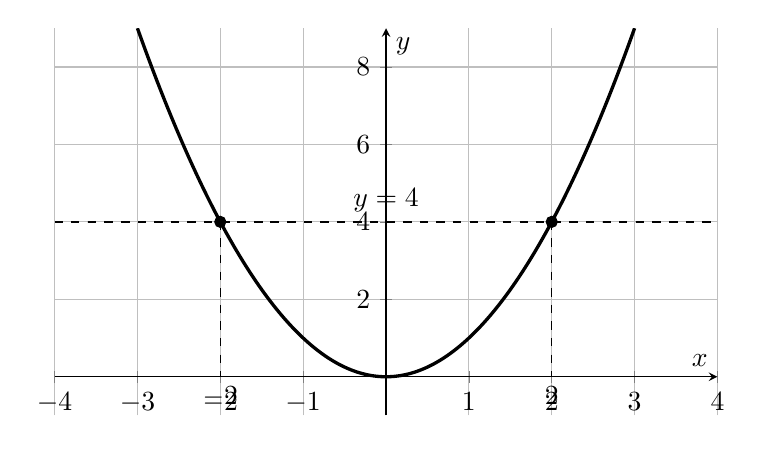
\begin{tikzpicture}
\begin{axis}[
    width=10cm,height=6.5cm,
    xmin=-4,xmax=4,ymin=-1,ymax=9,
    xlabel={$x$},ylabel={$y$},
    axis lines=middle,grid=both,samples=180
]
\addplot[very thick,domain=-3:3] {x^2};
\addplot[thick,dashed,domain=-4:4] {4};
\addplot[only marks,mark=*] coordinates {(-2,4)(2,4)};
\draw[dashed] (axis cs:-2,4)--(axis cs:-2,0);
\draw[dashed] (axis cs:2,4)--(axis cs:2,0);
\node[below] at (axis cs:-2,0) {$-2$};
\node[below] at (axis cs:2,0) {$2$};
\node[above] at (axis cs:0,4) {$y=4$};
\end{axis}
\end{tikzpicture}
\end{center}

De horizontale lijn \(y=4\) snijdt de grafiek tweemaal. De functiewaarde
\(4\) heeft dus twee originelen.
\end{voorbeeld}

Dit leidt tot onze eerste belangrijke voorwaarde: verschillende invoerwaarden
mogen niet op dezelfde uitvoerwaarde terechtkomen.

% ============================================================
% 2. INJECTIEF
% ============================================================

\FVDsection{Injectief: geen uitvoer dubbel gebruiken}

\begin{definitie}
Een functie \(f:A\to B\) heet \textbf{injectief} als verschillende
invoerwaarden verschillende beelden hebben.

Equivalent:
\[
f(x_1)=f(x_2)\Longrightarrow x_1=x_2.
\]
\end{definitie}

In de taal van originelen:

\begin{center}
\textbf{iedere functiewaarde heeft hoogstens één origineel.}
\end{center}

\begin{voorbeeld}[Injectief pijldiagram]

\begin{center}
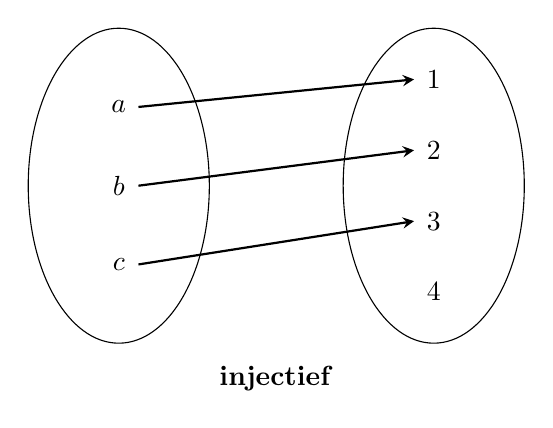
\begin{tikzpicture}[>=stealth]
\draw (-2,0) ellipse (1.15 and 2);
\draw (2,0) ellipse (1.15 and 2);
\node at (-2,1) {$a$};
\node at (-2,0) {$b$};
\node at (-2,-1) {$c$};
\node at (2,1.35) {$1$};
\node at (2,0.45) {$2$};
\node at (2,-0.45) {$3$};
\node at (2,-1.35) {$4$};
\draw[->,thick] (-1.75,1)--(1.75,1.35);
\draw[->,thick] (-1.75,0)--(1.75,0.45);
\draw[->,thick] (-1.75,-1)--(1.75,-0.45);
\node at (0,-2.45) {\textbf{injectief}};
\end{tikzpicture}
\end{center}

Geen enkel element rechts krijgt twee pijlen.
Element \(4\) wordt niet bereikt, maar dat verhindert injectiviteit niet.
\end{voorbeeld}

\begin{voorbeeld}[Niet injectief]

\begin{center}
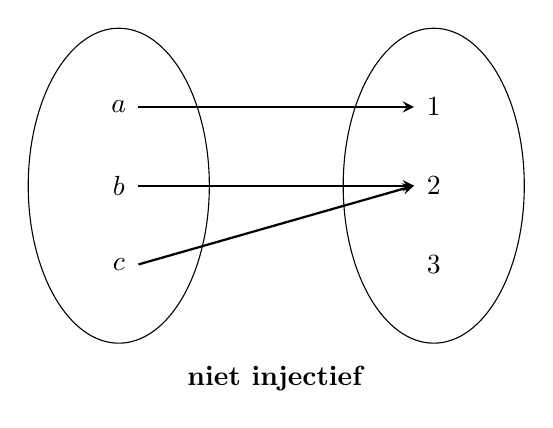
\begin{tikzpicture}[>=stealth]
\draw (-2,0) ellipse (1.15 and 2);
\draw (2,0) ellipse (1.15 and 2);
\node at (-2,1) {$a$};
\node at (-2,0) {$b$};
\node at (-2,-1) {$c$};
\node at (2,1) {$1$};
\node at (2,0) {$2$};
\node at (2,-1) {$3$};
\draw[->,thick] (-1.75,1)--(1.75,1);
\draw[->,thick] (-1.75,0)--(1.75,0);
\draw[->,thick] (-1.75,-1)--(1.75,0);
\node at (0,-2.45) {\textbf{niet injectief}};
\end{tikzpicture}
\end{center}

De uitvoer \(2\) heeft twee originelen, namelijk \(b\) en \(c\).
\end{voorbeeld}

% ============================================================
% 3. HORIZONTALE-LIJNTEST
% ============================================================

\FVDsubsection{Injectiviteit grafisch onderzoeken}

Bij het functiebegrip gebruikten we verticale lijnen. Nu willen we weten
hoeveel originelen een uitvoerwaarde heeft. Daarom gebruiken we
\textbf{horizontale} lijnen.

\begin{eigenschap}[Horizontale-lijntest]
Een functie is injectief als iedere horizontale lijn de grafiek
\textbf{hoogstens één keer} snijdt.
\end{eigenschap}

Waarom?

Een horizontale lijn
\[
y=b
\]
legt één functiewaarde \(b\) vast. De snijpunten met de grafiek geven precies
de originelen van \(b\).

\begin{center}
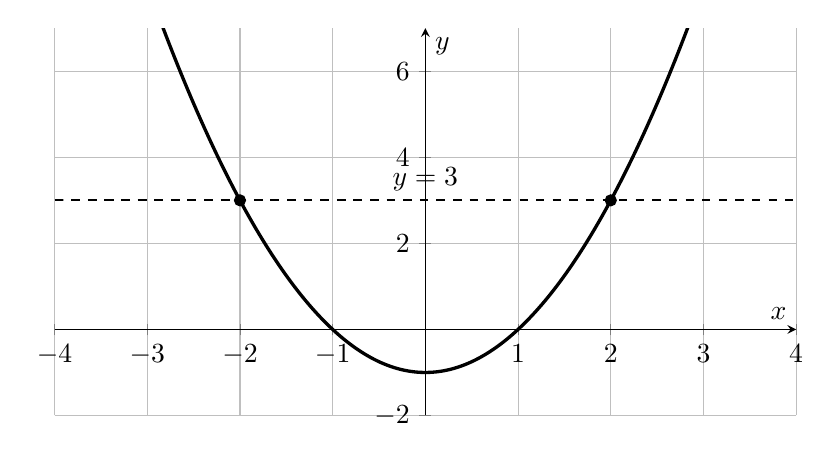
\begin{tikzpicture}
\begin{axis}[
    width=11cm,height=6.5cm,
    xmin=-4,xmax=4,ymin=-2,ymax=7,
    xlabel={$x$},ylabel={$y$},
    axis lines=middle,grid=both,samples=180
]
\addplot[very thick,domain=-3:3] {x^2-1};
\addplot[thick,dashed,domain=-4:4] {3};
\addplot[only marks,mark=*] coordinates {(-2,3)(2,3)};
\node[above] at (axis cs:0,3) {$y=3$};
\end{axis}
\end{tikzpicture}
\end{center}

De functie \(f(x)=x^2-1\) is op \(\mathbb R\) niet injectief:
de horizontale lijn \(y=3\) snijdt de grafiek tweemaal.

\begin{opmerking}[Niet verwarren]
\begin{itemize}
    \item \textbf{Verticale-lijntest}: is de relatie een functie?
    \item \textbf{Horizontale-lijntest}: is de functie injectief?
\end{itemize}

De twee tests beantwoorden dus verschillende vragen.
\end{opmerking}

% ============================================================
% 4. SURJECTIEF
% ============================================================

\FVDsection{Surjectief: wordt het volledige codomein bereikt?}

Injectiviteit gaat over \emph{hoeveel} originelen een uitvoerwaarde kan hebben.
Surjectiviteit gaat over de vraag of alle waarden die we als mogelijke uitvoer
hebben opgegeven ook werkelijk voorkomen.

\begin{definitie}
Een functie \(f:A\to B\) heet \textbf{surjectief} als ieder element van
het codomein \(B\) minstens één origineel heeft.
\end{definitie}

Equivalent:
\[
\boxed{\operatorname{ber}f=B.}
\]

\begin{center}
    \tikzset{every picture/.style={line width=0.75pt}} %set default line width to 0.75pt        

 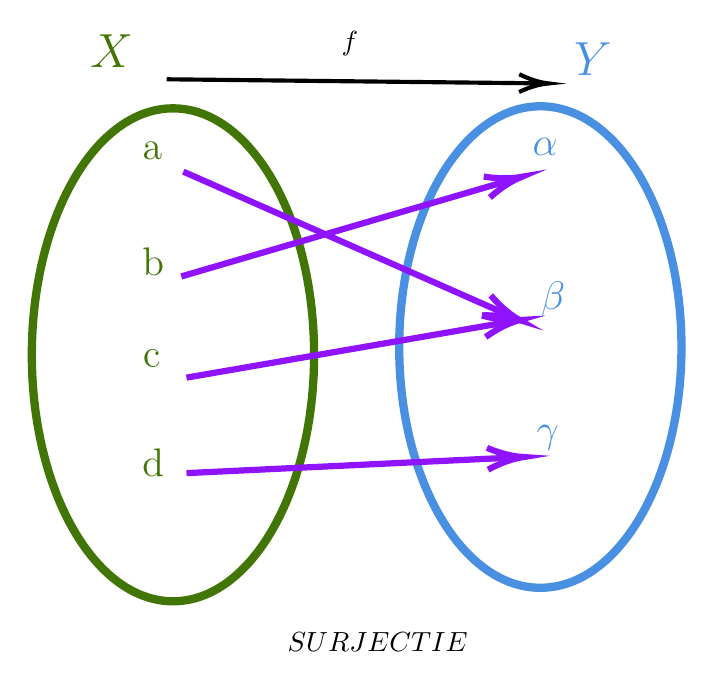
\begin{tikzpicture}[x=0.75pt,y=0.75pt,yscale=-1,xscale=1]
 %uncomment if require: \path (0,344); %set diagram left start at 0, and has height of 344

 %Shape: Ellipse [id:dp4304013190336202] 
 \draw  [color={rgb, 255:red, 74; green, 144; blue, 226 }  ,draw opacity=1 ][line width=3]  (196,160) .. controls (196,95.93) and (226.44,44) .. (264,44) .. controls (301.56,44) and (332,95.93) .. (332,160) .. controls (332,224.07) and (301.56,276) .. (264,276) .. controls (226.44,276) and (196,224.07) .. (196,160) -- cycle ;
 %Shape: Ellipse [id:dp268405774492684] 
 \draw  [color={rgb, 255:red, 65; green, 117; blue, 5 }  ,draw opacity=1 ][line width=3]  (19,163.75) .. controls (19,98.17) and (49.44,45) .. (87,45) .. controls (124.56,45) and (155,98.17) .. (155,163.75) .. controls (155,229.33) and (124.56,282.5) .. (87,282.5) .. controls (49.44,282.5) and (19,229.33) .. (19,163.75) -- cycle ;
 %Straight Lines [id:da5957709040712875] 
 \draw [color={rgb, 255:red, 144; green, 19; blue, 254 }  ,draw opacity=1 ][line width=2.25]    (91,126) -- (251.16,79.12) ;
 \draw [shift={(255,78)}, rotate = 163.69] [color={rgb, 255:red, 144; green, 19; blue, 254 }  ,draw opacity=1 ][line width=2.25]    (17.49,-5.26) .. controls (11.12,-2.23) and (5.29,-0.48) .. (0,0) .. controls (5.29,0.48) and (11.12,2.23) .. (17.49,5.26)   ;
 %Straight Lines [id:da5027721590356096] 
 \draw [color={rgb, 255:red, 144; green, 19; blue, 254 }  ,draw opacity=1 ][line width=2.25]    (92,75.5) -- (250.34,145.38) ;
 \draw [shift={(254,147)}, rotate = 203.81] [color={rgb, 255:red, 144; green, 19; blue, 254 }  ,draw opacity=1 ][line width=2.25]    (17.49,-5.26) .. controls (11.12,-2.23) and (5.29,-0.48) .. (0,0) .. controls (5.29,0.48) and (11.12,2.23) .. (17.49,5.26)   ;
 %Straight Lines [id:da3631155606631937] 
 \draw [color={rgb, 255:red, 0; green, 0; blue, 0 }  ,draw opacity=1 ][line width=1.5]    (84,31) -- (265,32.97) ;
 \draw [shift={(268,33)}, rotate = 180.62] [color={rgb, 255:red, 0; green, 0; blue, 0 }  ,draw opacity=1 ][line width=1.5]    (14.21,-4.28) .. controls (9.04,-1.82) and (4.3,-0.39) .. (0,0) .. controls (4.3,0.39) and (9.04,1.82) .. (14.21,4.28)   ;
 %Straight Lines [id:da3317706737203854] 
 \draw [color={rgb, 255:red, 144; green, 19; blue, 254 }  ,draw opacity=1 ][line width=2.25]    (93.5,174.75) -- (250.06,147.68) ;
 \draw [shift={(254,147)}, rotate = 170.19] [color={rgb, 255:red, 144; green, 19; blue, 254 }  ,draw opacity=1 ][line width=2.25]    (17.49,-5.26) .. controls (11.12,-2.23) and (5.29,-0.48) .. (0,0) .. controls (5.29,0.48) and (11.12,2.23) .. (17.49,5.26)   ;
 %Straight Lines [id:da48081546706207945] 
 \draw [color={rgb, 255:red, 144; green, 19; blue, 254 }  ,draw opacity=1 ][line width=2.25]    (93.5,220.75) -- (252,213.19) ;
 \draw [shift={(256,213)}, rotate = 177.27] [color={rgb, 255:red, 144; green, 19; blue, 254 }  ,draw opacity=1 ][line width=2.25]    (17.49,-5.26) .. controls (11.12,-2.23) and (5.29,-0.48) .. (0,0) .. controls (5.29,0.48) and (11.12,2.23) .. (17.49,5.26)   ;

 % Text Node
 \draw (46,8.4) node [anchor=north west][inner sep=0.75pt]  [font=\LARGE,color={rgb, 255:red, 65; green, 117; blue, 5 }  ,opacity=1 ]  {$X$};
 % Text Node
 \draw (279,12.4) node [anchor=north west][inner sep=0.75pt]  [font=\LARGE,color={rgb, 255:red, 74; green, 144; blue, 226 }  ,opacity=1 ]  {$Y$};
 % Text Node
 \draw (71,60) node [anchor=north west][inner sep=0.75pt]  [font=\Large,color={rgb, 255:red, 65; green, 117; blue, 5 }  ,opacity=1 ] [align=left] {a};
 % Text Node
 \draw (71,111) node [anchor=north west][inner sep=0.75pt]  [font=\Large,color={rgb, 255:red, 65; green, 117; blue, 5 }  ,opacity=1 ] [align=left] {b};
 % Text Node
 \draw (71,208) node [anchor=north west][inner sep=0.75pt]  [font=\Large,color={rgb, 255:red, 65; green, 117; blue, 5 }  ,opacity=1 ] [align=left] {d};
 % Text Node
 \draw (71.1,160.43) node [anchor=north west][inner sep=0.75pt]  [font=\Large,color={rgb, 255:red, 65; green, 117; blue, 5 }  ,opacity=1 ,rotate=-358.05] [align=left] {c};
 % Text Node
 \draw (141,296.4) node [anchor=north west][inner sep=0.75pt]    {$SURJECTIE$};
 % Text Node
 \draw (259,58.4) node [anchor=north west][inner sep=0.75pt]  [font=\Large,color={rgb, 255:red, 74; green, 144; blue, 226 }  ,opacity=1 ]  {$\alpha $};
 % Text Node
 \draw (263,127.4) node [anchor=north west][inner sep=0.75pt]  [font=\Large,color={rgb, 255:red, 74; green, 144; blue, 226 }  ,opacity=1 ]  {$\beta $};
 % Text Node
 \draw (261,196.4) node [anchor=north west][inner sep=0.75pt]  [font=\Large,color={rgb, 255:red, 74; green, 144; blue, 226 }  ,opacity=1 ]  {$\gamma $};
 % Text Node
 \draw (167,6.4) node [anchor=north west][inner sep=0.75pt]    {$f$};


 \end{tikzpicture}

\end{center}

\begin{voorbeeld}[Het codomein maakt verschil]

Beschouw
\[
f(x)=x^2.
\]

Als
\[
f:\mathbb R\to\mathbb R,
\]
dan is \(f\) niet surjectief: negatieve reële getallen worden niet bereikt.

Maar als
\[
f:\mathbb R\to[0,+\infty[,
\]
dan is \(f\) wel surjectief, want iedere niet-negatieve reële waarde is een
kwadraat van minstens één reëel getal.

Hetzelfde voorschrift kan dus, afhankelijk van het gekozen codomein,
wel of niet surjectief zijn.
\end{voorbeeld}



% ============================================================
% 5. BIJECTIEF
% ============================================================

\FVDsection{Bijectief: precies één origineel}

Nu kunnen we beide voorwaarden combineren.

\begin{definitie}
Een functie \(f:A\to B\) is \textbf{bijectief} als ze zowel injectief
als surjectief is.
\end{definitie}

Dat kunnen we veel betekenisvoller formuleren:

\begin{center}
\boxed{\text{Iedere waarde uit het codomein heeft precies één origineel.}}
\end{center}

\begin{center}
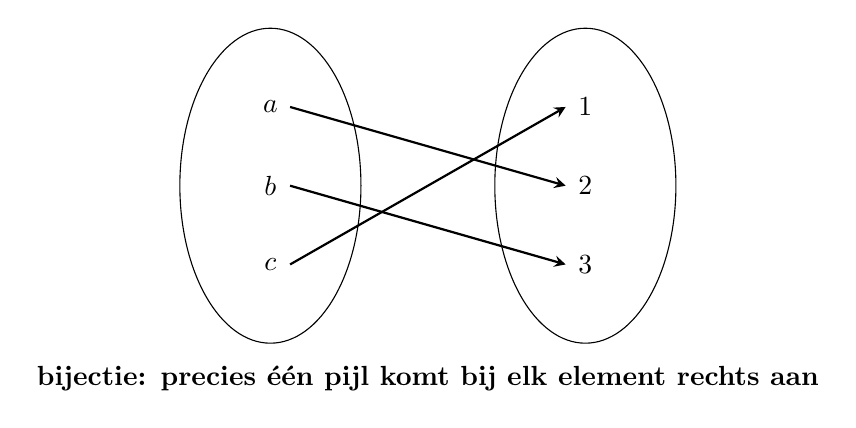
\begin{tikzpicture}[>=stealth]
\draw (-2,0) ellipse (1.15 and 2);
\draw (2,0) ellipse (1.15 and 2);
\node at (-2,1) {$a$};
\node at (-2,0) {$b$};
\node at (-2,-1) {$c$};
\node at (2,1) {$1$};
\node at (2,0) {$2$};
\node at (2,-1) {$3$};
\draw[->,thick] (-1.75,1)--(1.75,0);
\draw[->,thick] (-1.75,0)--(1.75,-1);
\draw[->,thick] (-1.75,-1)--(1.75,1);
\node at (0,-2.45) {\textbf{bijectie: precies één pijl komt bij elk element rechts aan}};
\end{tikzpicture}
\end{center}

Dit is precies wat we nodig hebben als we de functie willen omkeren.

\[
\boxed{
\text{bijectief}
\quad\Longleftrightarrow\quad
\text{iedere uitvoer heeft precies één origineel}
}
\]

\begin{voorbeeld}[Een lineaire functie]

Beschouw
\[
f:\mathbb R\to\mathbb R:x\mapsto 2x-3.
\]

De grafiek is een niet-horizontale rechte.

\begin{center}
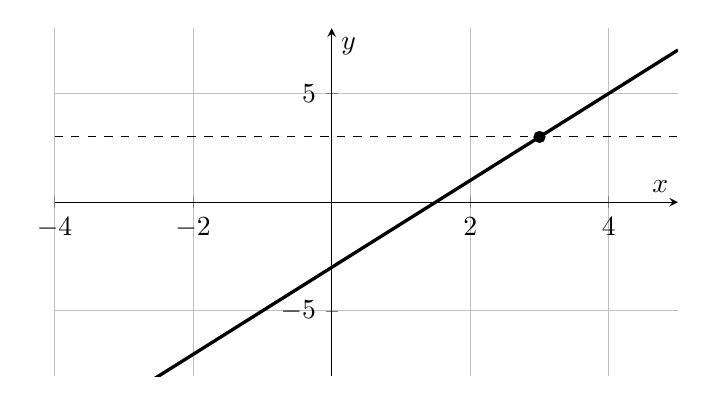
\begin{tikzpicture}
\begin{axis}[
    width=9.5cm,height=6cm,
    xmin=-4,xmax=5,ymin=-8,ymax=8,
    xlabel={$x$},ylabel={$y$},
    axis lines=middle,grid=both,samples=100
]
\addplot[very thick,domain=-3:5] {2*x-3};
\addplot[dashed,domain=-4:5] {3};
\addplot[only marks,mark=*] coordinates {(3,3)};
\end{axis}
\end{tikzpicture}
\end{center}

Iedere horizontale lijn snijdt de grafiek precies eenmaal.
Elke reële uitvoerwaarde heeft dus precies één reëel origineel.
De functie is bijectief.
\end{voorbeeld}

% ============================================================
% 6. DOMEIN BEPERKEN
% ============================================================

\FVDsection{Een functie omkeerbaar maken}

Een functie die op haar oorspronkelijke domein niet injectief is,
kan soms injectief worden door haar domein verstandig te beperken.

\begin{voorbeeld}[De kwadraatfunctie]

De functie
\[
f:\mathbb R\to[0,+\infty[:x\mapsto x^2
\]
is niet injectief, want bijvoorbeeld
\[
f(-2)=f(2).
\]

Beperk nu het domein:
\[
g:[0,+\infty[\to[0,+\infty[:x\mapsto x^2.
\]

\begin{center}
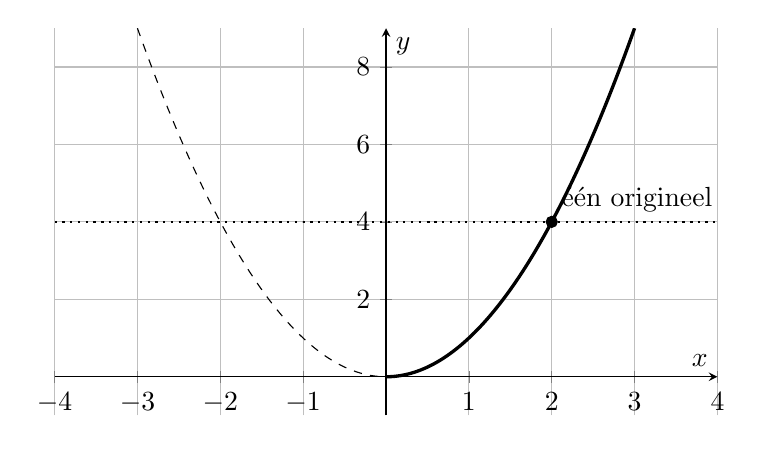
\begin{tikzpicture}
\begin{axis}[
    width=10cm,height=6.5cm,
    xmin=-4,xmax=4,ymin=-1,ymax=9,
    xlabel={$x$},ylabel={$y$},
    axis lines=middle,grid=both,samples=180
]
\addplot[dashed,domain=-3:0] {x^2};
\addplot[very thick,domain=0:3] {x^2};
\addplot[thick,dotted,domain=-4:4] {4};
\addplot[only marks,mark=*] coordinates {(2,4)};
\node[above right] at (axis cs:2,4) {één origineel in het gekozen domein};
\end{axis}
\end{tikzpicture}
\end{center}

Op het beperkte domein snijdt iedere horizontale lijn met \(y\geq0\)
de grafiek precies eenmaal. De functie \(g\) is dus bijectief.

We hadden ook het domein
\[
]-\infty,0]
\]
kunnen kiezen. Ook daar wordt de kwadraatfunctie bijectief naar
\([0,+\infty[\).
\end{voorbeeld}



% ============================================================
% 7. CODOMEIN AANPASSEN
% ============================================================

\FVDsubsection{Ook het codomein telt}

Bijectiviteit hangt niet alleen van het voorschrift af. Domein en codomein
maken deel uit van de functie.

Vergelijk:

\[
f:\mathbb R\to\mathbb R:x\mapsto x^2
\]

met

\[
g:[0,+\infty[\to[0,+\infty[:x\mapsto x^2.
\]

De eerste is noch injectief noch surjectief.
De tweede is zowel injectief als surjectief en dus bijectief.

\begin{center}
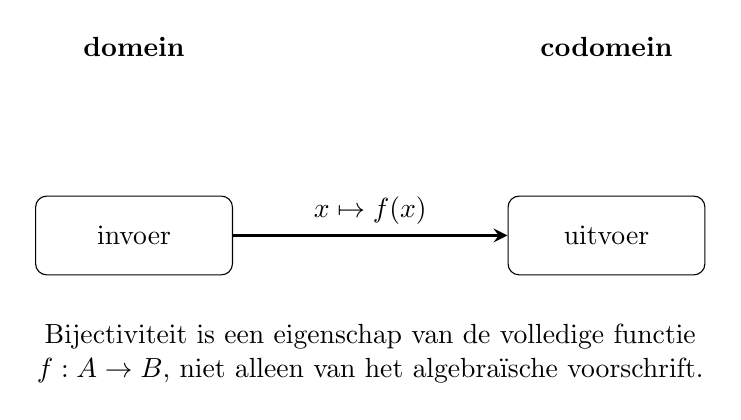
\begin{tikzpicture}[>=stealth]
\node at (-3,2.4) {\textbf{domein}};
\node at (3,2.4) {\textbf{codomein}};
\node[draw,rounded corners,minimum width=2.5cm,minimum height=1cm] (A) at (-3,0) {invoer};
\node[draw,rounded corners,minimum width=2.5cm,minimum height=1cm] (B) at (3,0) {uitvoer};
\draw[->,very thick] (A)--node[above] {\(x\mapsto f(x)\)}(B);
\node[align=center] at (0,-1.5) {Bijectiviteit is een eigenschap van de volledige functie\\
\(f:A\to B\), niet alleen van het algebraïsche voorschrift.};
\end{tikzpicture}
\end{center}

% ============================================================
% 8. GEOGEBRA-ONDERZOEK
% ============================================================

\FVDsubsection{Omkeerbaarheid onderzoeken met GeoGebra}

\begin{fvdgeogebra}[Injectiviteit onderzoeken met een horizontale lijn]

    Voer in GeoGebra de functies
    
    \[
    f(x)=x^2,
    \qquad
    g(x)=x^3,
    \qquad
    h(x)=|x|.
    \]
    
    Maak een schuifknop \(b\) en teken de horizontale lijn
    
    \[
    y=b.
    \]
    
    Beweeg de schuifknop en onderzoek voor elke functie:
    
    \begin{enumerate}
    
        \item Hoeveel snijpunten kan de lijn \(y=b\) met de grafiek hebben?
    
        \item Welke functies zijn op \(\mathbb{R}\) injectief?
    
        \item Welke functiewaarden hebben geen, precies één of meerdere
              originelen?
    
        \item Hoe kan je het domein van \(f(x)=x^2\) beperken zodat elke
              functiewaarde hoogstens één origineel heeft?
    
        \item Kan je het domein van \(h(x)=|x|\) op een gelijkaardige manier
              beperken? Geef twee mogelijke keuzes.
    
    \end{enumerate}
    
    Formuleer eerst een vermoeden op basis van de grafiek en verantwoord
    daarna je besluit vanuit de definitie van injectiviteit.
    
    \end{fvdgeogebra}

% ============================================================
% 9. STEM
% ============================================================

\FVDsubsection{Toepassingen}

In toepassingen gebruiken we functies vaak als omzettingen.

\begin{voorbeeld}[Een lineaire temperatuursensor]

Een temperatuursensor wordt in zijn werkgebied beschreven door
\[
U(T)=0{,}50+0{,}020T,
\qquad -20\leq T\leq80.
\]

Het bereik is
\[
0{,}10\leq U\leq2{,}10.
\]

Beschouwen we
\[
U:[-20,80]\to[0{,}10,2{,}10],
\]
dan heeft iedere toegelaten spanning precies één bijbehorende temperatuur.

De omzetting is dus bijectief.

Dat is praktisch belangrijk: uit een gemeten uitgangsspanning kunnen we
eenduidig de temperatuur terugvinden.

\begin{center}
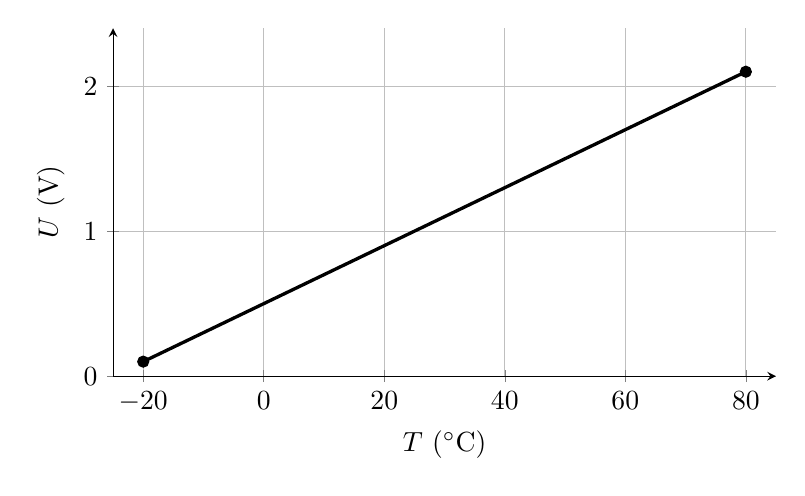
\begin{tikzpicture}
\begin{axis}[
    width=10cm,height=6cm,
    xmin=-25,xmax=85,ymin=0,ymax=2.4,
    xlabel={$T$ ($^\circ$C)},ylabel={$U$ (V)},
    axis lines=left,grid=both,samples=100
]
\addplot[very thick,domain=-20:80] {0.5+0.02*x};
\addplot[only marks,mark=*] coordinates {(-20,0.1)(80,2.1)};
\end{axis}
\end{tikzpicture}
\end{center}
\end{voorbeeld}

\begin{voorbeeld}[Een sensor die informatie verliest]

Stel dat een sensor een grootheid \(x\) omzet volgens
\[
S(x)=x^2
\qquad\text{voor}\qquad -5\leq x\leq5.
\]

Een uitlezing \(S=9\) kan afkomstig zijn van
\[
x=-3
\qquad\text{of}\qquad
x=3.
\]

De omzetting verliest dus informatie over het teken van de oorspronkelijke
waarde. Zonder bijkomende informatie kan de invoer niet eenduidig worden
gereconstrueerd.

Dit is precies het probleem van niet-injectiviteit.
\end{voorbeeld}

% ============================================================
% 10. SAMENVATTING
% ============================================================

\FVDsection{Samenvatting}

\begin{center}
\begin{tabular}{c|c|c}
\textbf{eigenschap} & \textbf{originelen} & \textbf{grafische betekenis}\\
\hline
injectief & hoogstens één & horizontale lijn snijdt hoogstens eenmaal\\
surjectief & minstens één voor elk element codomein & bereik = codomein\\
bijectief & precies één voor elk element codomein & eenduidige terugweg
\end{tabular}
\end{center}



\end{document}

